% Elementos del grupo diédrico D4 actuando sobre un patch 3x3
% Compilar con: pdflatex d4_group_actions.tex
\documentclass[tikz,border=10pt]{standalone}
\usepackage{tikz}
\usepackage{amsmath,amssymb}
\usetikzlibrary{positioning}

\definecolor{gdlblue}{RGB}{41, 98, 168}
\definecolor{gdlred}{RGB}{191, 49, 49}
\definecolor{gdlgreen}{RGB}{30, 130, 76}
\definecolor{gdlorange}{RGB}{217, 130, 30}
\definecolor{gdlpurple}{RGB}{118, 56, 138}
\definecolor{gdlgray}{RGB}{140, 140, 140}
\definecolor{gdlyellow}{RGB}{190, 140, 10}

\begin{document}
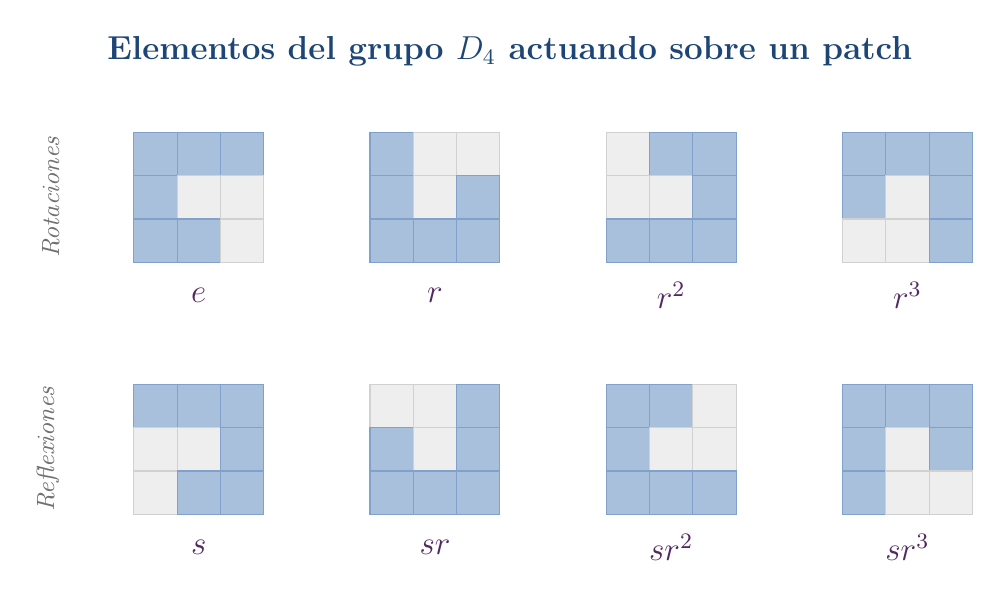
\begin{tikzpicture}[
    filled/.style={minimum size=0.55cm, inner sep=0pt, outer sep=0pt,
                   fill=gdlblue!40, draw=gdlblue!60},
    empty/.style={minimum size=0.55cm, inner sep=0pt, outer sep=0pt,
                  fill=gdlgray!15, draw=gdlgray!40},
    grouplabel/.style={font=\large, text=gdlpurple!70!black},
    rowlabel/.style={font=\small\itshape, text=gdlgray!80!black, rotate=90, anchor=south},
    title/.style={font=\large\bfseries, text=gdlblue!70!black}
]

% Cell size
\def\cs{0.55}
% Horizontal spacing between patch centers
\def\hs{3.0}
% Vertical spacing between row centers
\def\vs{3.2}

% Macro: draw a 3x3 patch
% #1 = x offset, #2 = y offset
% #3-#11 = 9 cell values (1=filled, 0=empty), row by row top to bottom, left to right
\newcommand{\patch}[7]{%
    % Parse the 9-character string #3 as a grid
    % We'll use individual cell commands instead
    \begin{scope}[shift={(#1,#2)}]
        \patchcell{0}{0}{#3}\patchcell{1}{0}{#4}\patchcell{2}{0}{#5}%
        \patchcell{0}{1}{#6}\patchcell{1}{1}{#7}%
    \end{scope}
}
% This macro approach is complex; let's use explicit node placement instead.

% === Utility: draw one cell ===
% #1=col, #2=row-from-top, #3=xoff, #4=yoff, #5=style(filled/empty)
\newcommand{\cell}[5]{%
    \node[#5] at ({#3 + #1*\cs}, {#4 - #2*\cs}) {};%
}

% === Macro to draw a full 3x3 grid + label ===
% #1=xoff, #2=yoff, #3=label text
% #4#5#6 = row0 (3 chars, each f or e)
% #7#8#9 = row1
% #10#11#12 = row2
% Too many args; let's just do it explicitly below.

% ---------- Title ----------
\node[title] at ({1.5*\hs}, {1.3}) {Elementos del grupo $D_4$ actuando sobre un patch};

% ============================================================
% TOP ROW: Rotations
% ============================================================

% --- e (identity) ---
% Pattern "F":
%   1 1 1
%   1 0 0
%   1 1 0
\begin{scope}[shift={(0, 0)}]
    \node[filled] at (0,     0)     {};  % (0,0)
    \node[filled] at (\cs,   0)     {};  % (0,1)
    \node[filled] at (2*\cs, 0)     {};  % (0,2)
    \node[filled] at (0,    -\cs)   {};  % (1,0)
    \node[empty]  at (\cs,  -\cs)   {};  % (1,1)
    \node[empty]  at (2*\cs,-\cs)   {};  % (1,2)
    \node[filled] at (0,    -2*\cs) {};  % (2,0)
    \node[filled] at (\cs,  -2*\cs) {};  % (2,1)
    \node[empty]  at (2*\cs,-2*\cs) {};  % (2,2)
    \node[grouplabel] at (\cs, -2*\cs - 0.7) {$e$};
\end{scope}

% --- r (90° CCW) ---
%   1 0 0
%   1 0 1
%   1 1 1
\begin{scope}[shift={(\hs, 0)}]
    \node[filled] at (0,     0)     {};
    \node[empty]  at (\cs,   0)     {};
    \node[empty]  at (2*\cs, 0)     {};
    \node[filled] at (0,    -\cs)   {};
    \node[empty]  at (\cs,  -\cs)   {};
    \node[filled] at (2*\cs,-\cs)   {};
    \node[filled] at (0,    -2*\cs) {};
    \node[filled] at (\cs,  -2*\cs) {};
    \node[filled] at (2*\cs,-2*\cs) {};
    \node[grouplabel] at (\cs, -2*\cs - 0.7) {$r$};
\end{scope}

% --- r² (180°) ---
%   0 1 1
%   0 0 1
%   1 1 1
\begin{scope}[shift={(2*\hs, 0)}]
    \node[empty]  at (0,     0)     {};
    \node[filled] at (\cs,   0)     {};
    \node[filled] at (2*\cs, 0)     {};
    \node[empty]  at (0,    -\cs)   {};
    \node[empty]  at (\cs,  -\cs)   {};
    \node[filled] at (2*\cs,-\cs)   {};
    \node[filled] at (0,    -2*\cs) {};
    \node[filled] at (\cs,  -2*\cs) {};
    \node[filled] at (2*\cs,-2*\cs) {};
    \node[grouplabel] at (\cs, -2*\cs - 0.7) {$r^2$};
\end{scope}

% --- r³ (270° CCW) ---
%   1 1 1
%   1 0 1
%   0 0 1
\begin{scope}[shift={(3*\hs, 0)}]
    \node[filled] at (0,     0)     {};
    \node[filled] at (\cs,   0)     {};
    \node[filled] at (2*\cs, 0)     {};
    \node[filled] at (0,    -\cs)   {};
    \node[empty]  at (\cs,  -\cs)   {};
    \node[filled] at (2*\cs,-\cs)   {};
    \node[empty]  at (0,    -2*\cs) {};
    \node[empty]  at (\cs,  -2*\cs) {};
    \node[filled] at (2*\cs,-2*\cs) {};
    \node[grouplabel] at (\cs, -2*\cs - 0.7) {$r^3$};
\end{scope}

% Row label
\node[rowlabel] at (-1.1, -\cs) {Rotaciones};

% ============================================================
% BOTTOM ROW: Reflections
% ============================================================

% --- s (vertical axis reflection) ---
%   1 1 1
%   0 0 1
%   0 1 1
\begin{scope}[shift={(0, -\vs)}]
    \node[filled] at (0,     0)     {};
    \node[filled] at (\cs,   0)     {};
    \node[filled] at (2*\cs, 0)     {};
    \node[empty]  at (0,    -\cs)   {};
    \node[empty]  at (\cs,  -\cs)   {};
    \node[filled] at (2*\cs,-\cs)   {};
    \node[empty]  at (0,    -2*\cs) {};
    \node[filled] at (\cs,  -2*\cs) {};
    \node[filled] at (2*\cs,-2*\cs) {};
    \node[grouplabel] at (\cs, -2*\cs - 0.7) {$s$};
\end{scope}

% --- sr ---
%   0 0 1
%   1 0 1
%   1 1 1
\begin{scope}[shift={(\hs, -\vs)}]
    \node[empty]  at (0,     0)     {};
    \node[empty]  at (\cs,   0)     {};
    \node[filled] at (2*\cs, 0)     {};
    \node[filled] at (0,    -\cs)   {};
    \node[empty]  at (\cs,  -\cs)   {};
    \node[filled] at (2*\cs,-\cs)   {};
    \node[filled] at (0,    -2*\cs) {};
    \node[filled] at (\cs,  -2*\cs) {};
    \node[filled] at (2*\cs,-2*\cs) {};
    \node[grouplabel] at (\cs, -2*\cs - 0.7) {$sr$};
\end{scope}

% --- sr² ---
%   1 1 0
%   1 0 0
%   1 1 1
\begin{scope}[shift={(2*\hs, -\vs)}]
    \node[filled] at (0,     0)     {};
    \node[filled] at (\cs,   0)     {};
    \node[empty]  at (2*\cs, 0)     {};
    \node[filled] at (0,    -\cs)   {};
    \node[empty]  at (\cs,  -\cs)   {};
    \node[empty]  at (2*\cs,-\cs)   {};
    \node[filled] at (0,    -2*\cs) {};
    \node[filled] at (\cs,  -2*\cs) {};
    \node[filled] at (2*\cs,-2*\cs) {};
    \node[grouplabel] at (\cs, -2*\cs - 0.7) {$sr^2$};
\end{scope}

% --- sr³ ---
%   1 1 1
%   1 0 1
%   1 0 0
\begin{scope}[shift={(3*\hs, -\vs)}]
    \node[filled] at (0,     0)     {};
    \node[filled] at (\cs,   0)     {};
    \node[filled] at (2*\cs, 0)     {};
    \node[filled] at (0,    -\cs)   {};
    \node[empty]  at (\cs,  -\cs)   {};
    \node[filled] at (2*\cs,-\cs)   {};
    \node[filled] at (0,    -2*\cs) {};
    \node[empty]  at (\cs,  -2*\cs) {};
    \node[empty]  at (2*\cs,-2*\cs) {};
    \node[grouplabel] at (\cs, -2*\cs - 0.7) {$sr^3$};
\end{scope}

% Row label
\node[rowlabel] at (-1.1, -\vs - \cs) {Reflexiones};

\end{tikzpicture}
\end{document}
